%% First draft. Every figure is drawn by ../figures.py from ../results.csv and is
%% stamped PLACEHOLDER while any row it draws is a dummy. Build: tectonic main.tex
\documentclass[sigconf,anonymous]{aamas}

\makeatletter
\gdef\@copyrightpermission{
  \begin{minipage}{0.2\columnwidth}
   \href{https://creativecommons.org/licenses/by/4.0/}{
\includegraphics[width=0.90\textwidth]{by}}
  \end{minipage}\hfill
  \begin{minipage}{0.8\columnwidth}
   \href{https://creativecommons.org/licenses/by/4.0/}{This work is licensed under a Creative Commons Attribution International 4.0 License.}
  \end{minipage}
  \vspace{5pt}
}
\makeatother

\setcopyright{ifaamas}
\acmConference[AAMAS 2027]{Proc.\@ of the 26th International Conference
on Autonomous Agents and Multiagent Systems (AAMAS 2027)}{3--7 May 2027}{Hanoi, Vietnam}{M.~Baldoni, F.~Fang, W.~Yeoh, N.~Yorke-Smith (eds.)}
\copyrightyear{2027}
\acmYear{2027}
\acmDOI{}
\acmISBN{}
\acmSubmissionID{<<OpenReview submission id>>}
\submissionType{Research Paper Track}

\newcommand{\todo}[1]{\textcolor{red}{[TODO: #1]}}
\newcommand{\gates}{G.A.T.E.S.}

\title{\gates: A Portable Validity Layer for Autonomous Research Agents}

\author{Keshav Jindal}
\affiliation{
  \institution{\todo{affiliation}}
  \country{\todo{country}}}

\begin{abstract}
Autonomous research agents publish numbers their experiments never produced.
The usual explanation is that the model fabricates.
In the scaffold we audited, the cause was mechanical: experiment output was truncated to 1,000 characters before any agent read it, so the writer could not see the real numbers and the failure detector could not see the crash.
We treat hallucinated results as an information-flow defect and close the channel at three points: execution validity, source-result coherence and report validity.
The three gates are deterministic, need no model to reach a verdict, and install into an existing scaffold through one small adapter.
A single switch runs them cumulatively, so each gate's contribution can be measured on its own.
We evaluate the layer on CORE-Bench, MLR-Bench and BadScientist at every level, on two host scaffolds.
\todo{one sentence of headline results, from the level-3 bars of Figures 1--3, once measured.}
\end{abstract}

\keywords{autonomous research agents, scientific integrity, hallucination, verification}

\begin{document}

\pagestyle{fancy}
\fancyhead{}

\maketitle

\section{Introduction}

Research agents such as Agent Laboratory~\cite{schmidgall2025agentlab} and The AI Scientist-v2~\cite{yamada2025aiscientistv2} run experiments and write the papers that report them.
Their papers regularly state results that no experiment produced: MLR-Bench found faked experimental results in every one of the ten papers AI Scientist-v2 wrote for its experimentation tasks~\cite{chen2025mlrbench}.

In the Agent Laboratory scaffold we audited, the mechanism was mundane.
Experiment output was truncated to 1,000 characters before the writing agent read it, and the crash marker was appended \emph{after} the program's own output, so it fell off the end of the same slice.
A run that raised \texttt{NameError} on every attempt was scored 1.0 by the reward model and written up with a full results table.
The model did not need to be dishonest; it was never shown the numbers.

That makes fabrication a property of the information flow, and so something a deterministic layer can stop.
\gates{} places a gate at each point where a scaffold loses its grip on evidence:

\begin{itemize}
\item \textbf{Gate 1, execution validity.} Did the code run, and did \emph{this} run produce the numbers? Only values the experiment recorded become citable.
\item \textbf{Gate 2, source-result coherence.} Is the verified run consistent with the ranges, relations and methodology its plan declared?
\item \textbf{Gate 3, report validity.} Is every number in the manuscript rendered from a recorded value, and does every citation resolve to a paper the run retrieved?
\end{itemize}

Our contributions are:
(1) the three gates, whose verdicts no model can change;
(2) a cumulative switch that runs them one at a time, so each gate's effect is measured rather than assumed;
(3) an install path shipped as agent skills, one per gate, tested against the code it describes;
and (4) an evaluation on three benchmarks, at every level, on two hosts.

\section{Related Work}

\paragraph{Research agents.}
Agent Laboratory~\cite{schmidgall2025agentlab} and The AI Scientist-v2~\cite{yamada2025aiscientistv2} automate the path from idea to paper.
ScientistOne~\cite{scientistone2026} maintains chains of evidence through its own pipeline, and audits other systems' released papers after the fact with four checks.
Three of them correspond to our gates: score verification to Gate 1, specification violation to Gate 2, and reference verification to Gate 3.
The difference is where the check sits: \gates{} runs inside an existing scaffold, before the paper exists, and sends each rejection back to the agent as feedback.

\paragraph{Benchmarks.}
MLR-Bench~\cite{chen2025mlrbench} evaluates agents on open-ended machine-learning research and labels the hallucinations in their papers.
CORE-Bench~\cite{siegel2024corebench} asks agents to reproduce published code and answer questions about its outputs.
BadScientist~\cite{jiang2025badscientist} shows that fabricated papers with no experiments are accepted by LLM reviewers at high rates under presentation-level manipulation.

\section{The Validity Layer}

\subsection{Design invariants}

The layer is Python-standard-library-only and imports nothing from the host.
Deterministic checks decide every verdict; a model can add a warning and nothing else, because the function that records a model's finding fixes its severity at WARN.
A check with no input emits nothing rather than passing, so a report never shows a green row for a check that did not run.
A gate never modifies what it judges; it writes its evidence beside it.

\subsection{Exhaustion policy}

Each gate runs a feedback loop with a budget counted in agent turns.
The policies on a spent budget differ on purpose (Table~\ref{tab:exhaustion}): a genuine novel result must not be blocked forever by Gate 2, while an unverifiable experiment or manuscript must not be emitted.

\begin{table}[t]
\caption{What each gate does when its budget is spent.}
\label{tab:exhaustion}
\begin{tabular}{p{0.36\columnwidth}p{0.56\columnwidth}}
\toprule
Gate & On exhaustion \\
\midrule
1 Execution validity & raise: no valid experiment, no paper \\
2 Source-result coherence & proceed, discrepancies declared as limitations \\
3 Report validity & raise: an unverifiable manuscript is not emitted \\
\bottomrule
\end{tabular}
\end{table}

\subsection{Cumulative levels}

One environment variable, \texttt{GATES\_LEVEL}, selects 0 (all off), 1 (Gate 1), 2 (Gates 1 and 2) or 3 (all three).
The levels are cumulative because each gate reads what the one before it produced: Gate 2 reviews Gate 1's registry, and Gate 3 judges a manuscript against it.
A closed gate raises before it spends an agent turn, so no setting runs a gate without the ones below it.

\section{Installing into a Host}

The loops every host shares live in the layer itself.
A host adapter supplies only host knowledge: a context per phase, its model call, its original execution path for level 0, and the ids of the papers it retrieved.
For Agent Laboratory that adapter is \todo{line count once frozen} lines.
The install path ships as four agent skills: a router and one skill per gate, each naming what it needs from the gate before it and what it hands on.
\todo{Phase 7: the AI Scientist-v2 adapter, and how many turns an agent took to write it from the skills.}

\section{Evaluation Protocol}

We run each host at all four levels on three benchmarks, and report one integrity metric and one task score for each (Table~\ref{tab:metrics}).
Pairing the two follows ScientistOne's framing: integrity should rise without the task score falling.
Every rate carries a Wilson interval and its denominator; published numbers carry neither.

\begin{table*}[t]
\caption{Metrics, and which gate has input on which benchmark. A gate with no input emits nothing, so its bar repeats the level below it.}
\label{tab:metrics}
\begin{tabular}{llll}
\toprule
Benchmark & Integrity metric (lower is better) & Task score (higher is better) & Gate with no input \\
\midrule
CORE-Bench (Hard, 45 tasks) & answers not traceable to a recorded value & pass@1 & Gate 3: no manuscript \\
MLR-Bench (10 tasks) & papers with faked experimental results & MLR-Judge overall & none \\
BadScientist (40 write-ups) & manipulated manuscripts emitted and accepted & honest manuscripts admitted & none \\
\bottomrule
\end{tabular}
\end{table*}

For BadScientist we manipulate the write-ups of real runs rather than generating papers with no experiments.
A paper with no experiment never passes Gate 1, so every level from 1 up would read zero and say nothing about Gates 2 and 3.
The faked-result labels come from a judge that is not the model under test.

\section{Results}

\todo{Every figure in this section is a dummy showing the expected shape. Replace from ../results.csv; see ../PLAN.md section 5.}

\begin{figure*}[t]
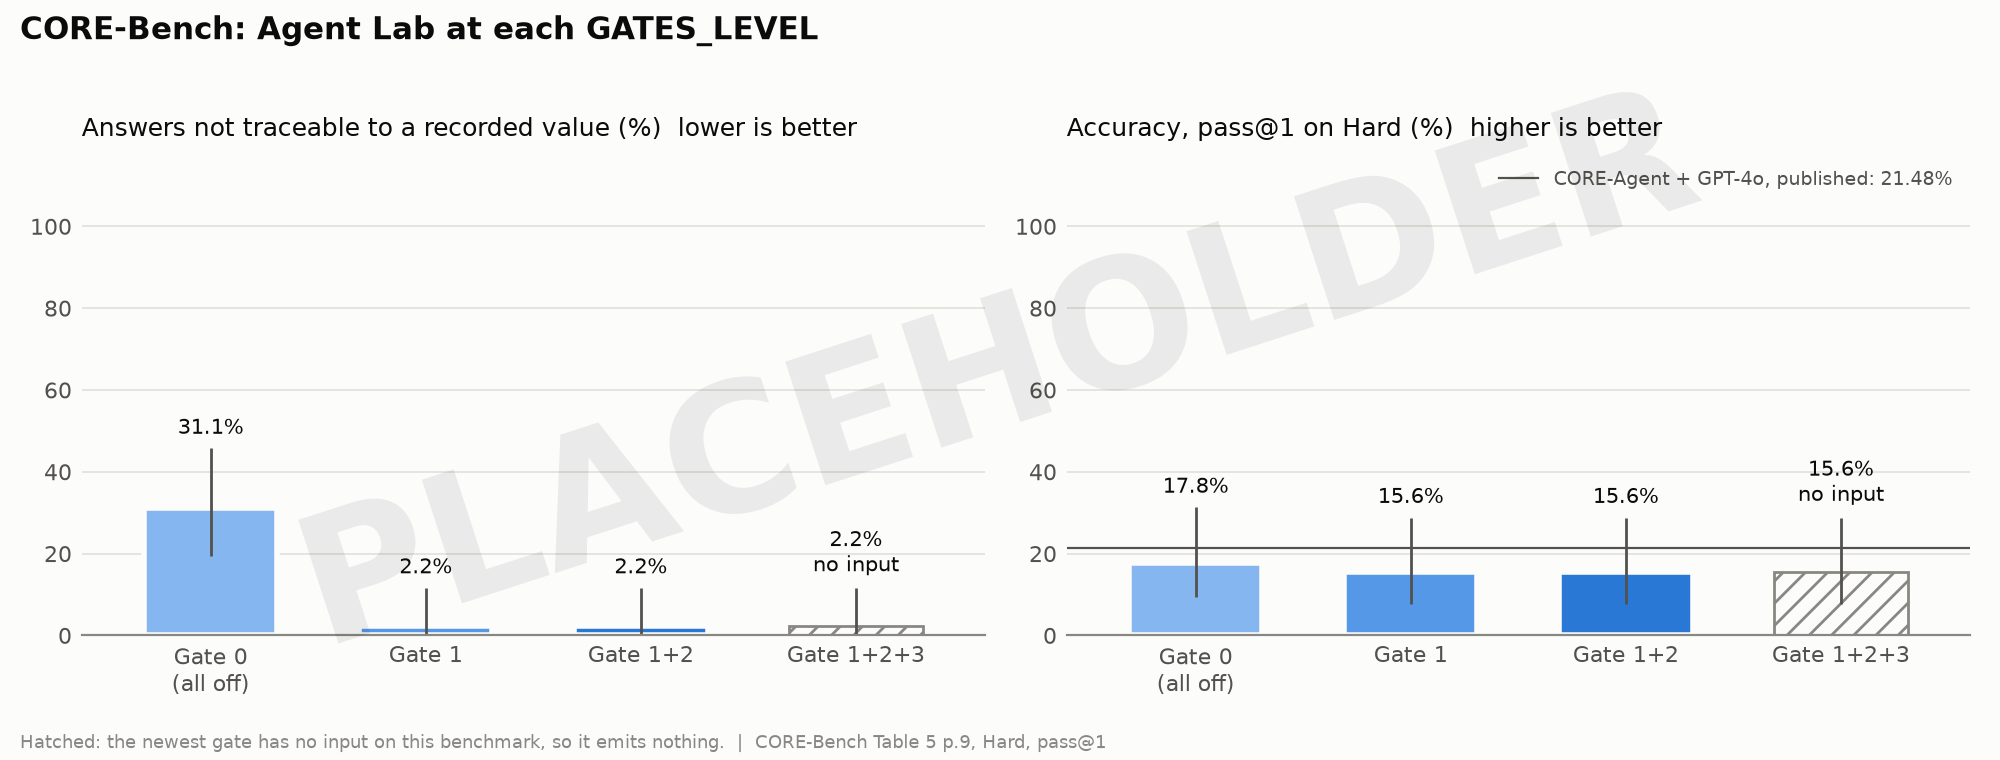
\includegraphics[width=\textwidth]{../figures/fig1_corebench_levels.png}
\caption{CORE-Bench by level. Gate 3 has no manuscript to read, so its bar is hatched.}
\label{fig:core}
\end{figure*}

\begin{figure*}[t]
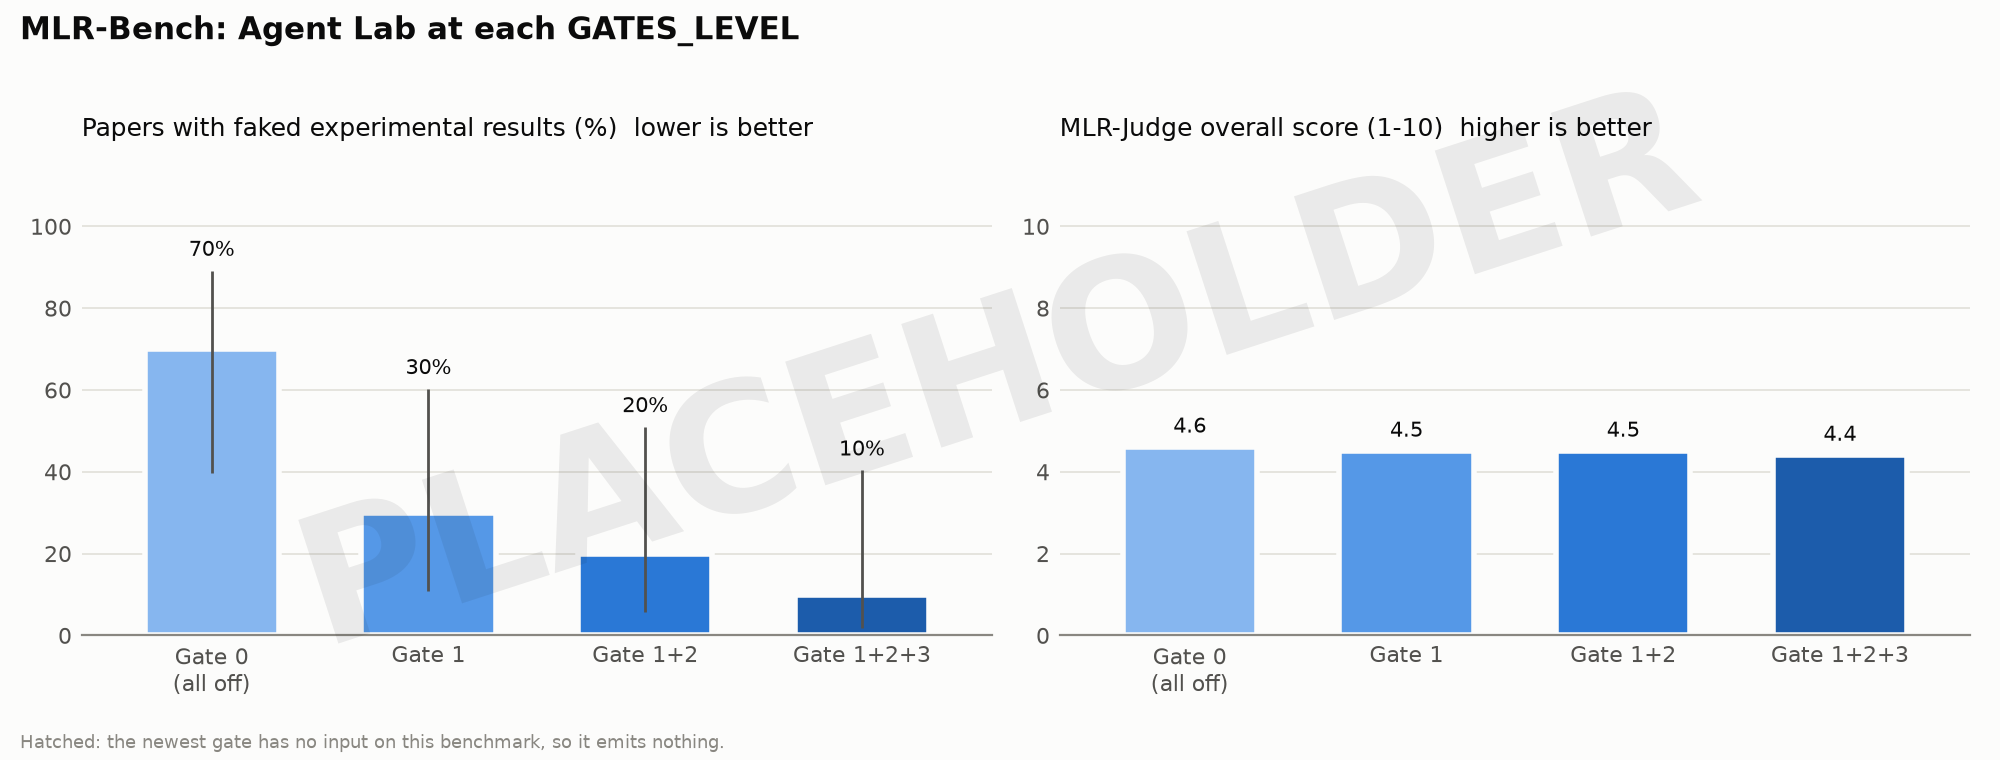
\includegraphics[width=\textwidth]{../figures/fig2_mlrbench_levels.png}
\caption{MLR-Bench by level.}
\label{fig:mlr}
\end{figure*}

\begin{figure*}[t]
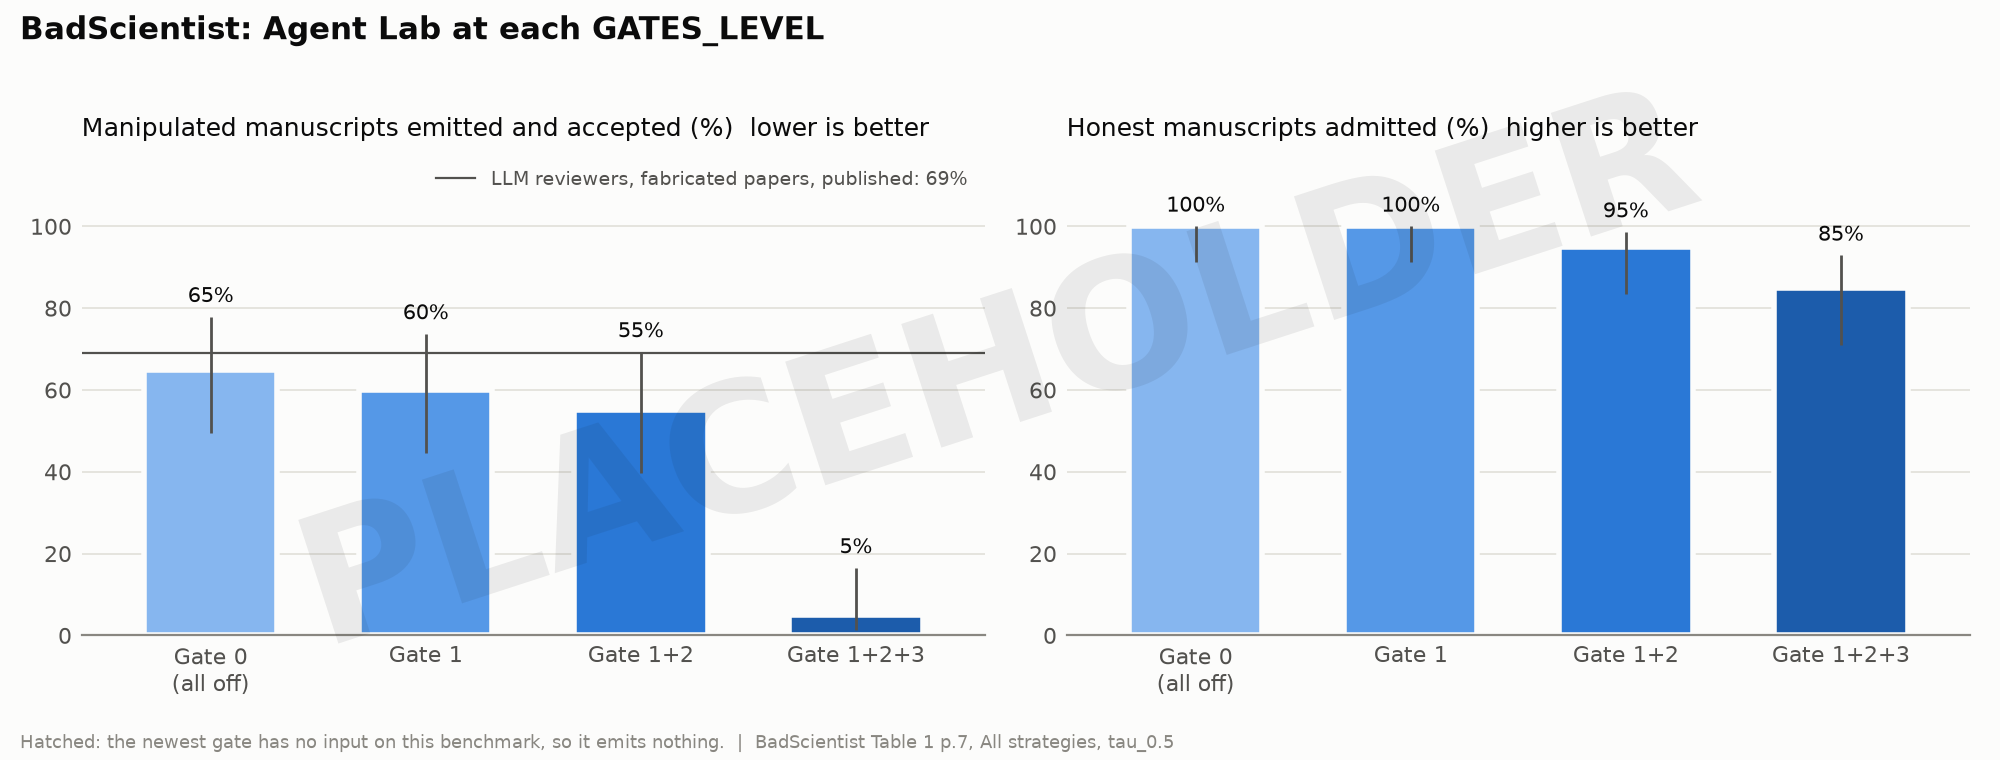
\includegraphics[width=\textwidth]{../figures/fig3_badscientist_levels.png}
\caption{BadScientist by level. The attack lives in the write-up, so Gate 3 is expected to carry this result.}
\label{fig:bad}
\end{figure*}

\paragraph{Each gate's contribution.}
\todo{Figures~\ref{fig:core}--\ref{fig:bad}: where the integrity metric drops, and whether the task score moved.}

\begin{figure*}[t]
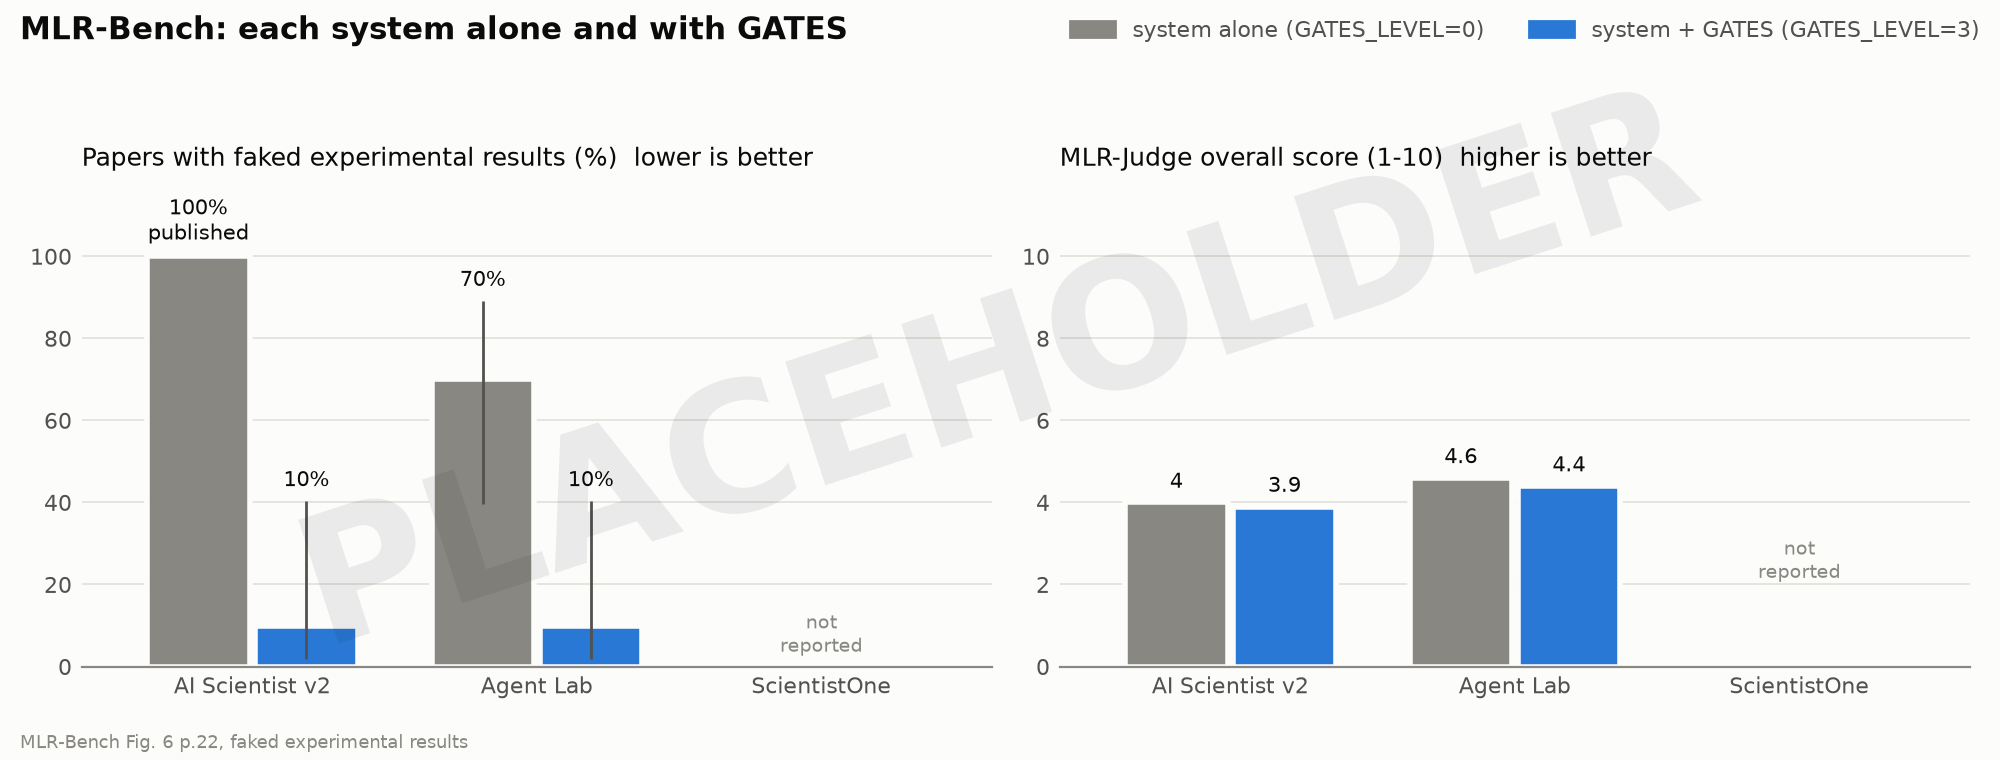
\includegraphics[width=\textwidth]{../figures/fig5_mlrbench_compare.png}
\caption{Each system alone (level 0) and with \gates{} (level 3) on MLR-Bench. AI Scientist-v2 alone is MLR-Bench's published figure. CORE-Bench and BadScientist are in the appendix.}
\label{fig:compare}
\end{figure*}

\paragraph{Across hosts.}
\todo{Figure~\ref{fig:compare}: host alone against host with \gates{}.}

\begin{figure*}[t]
\centering
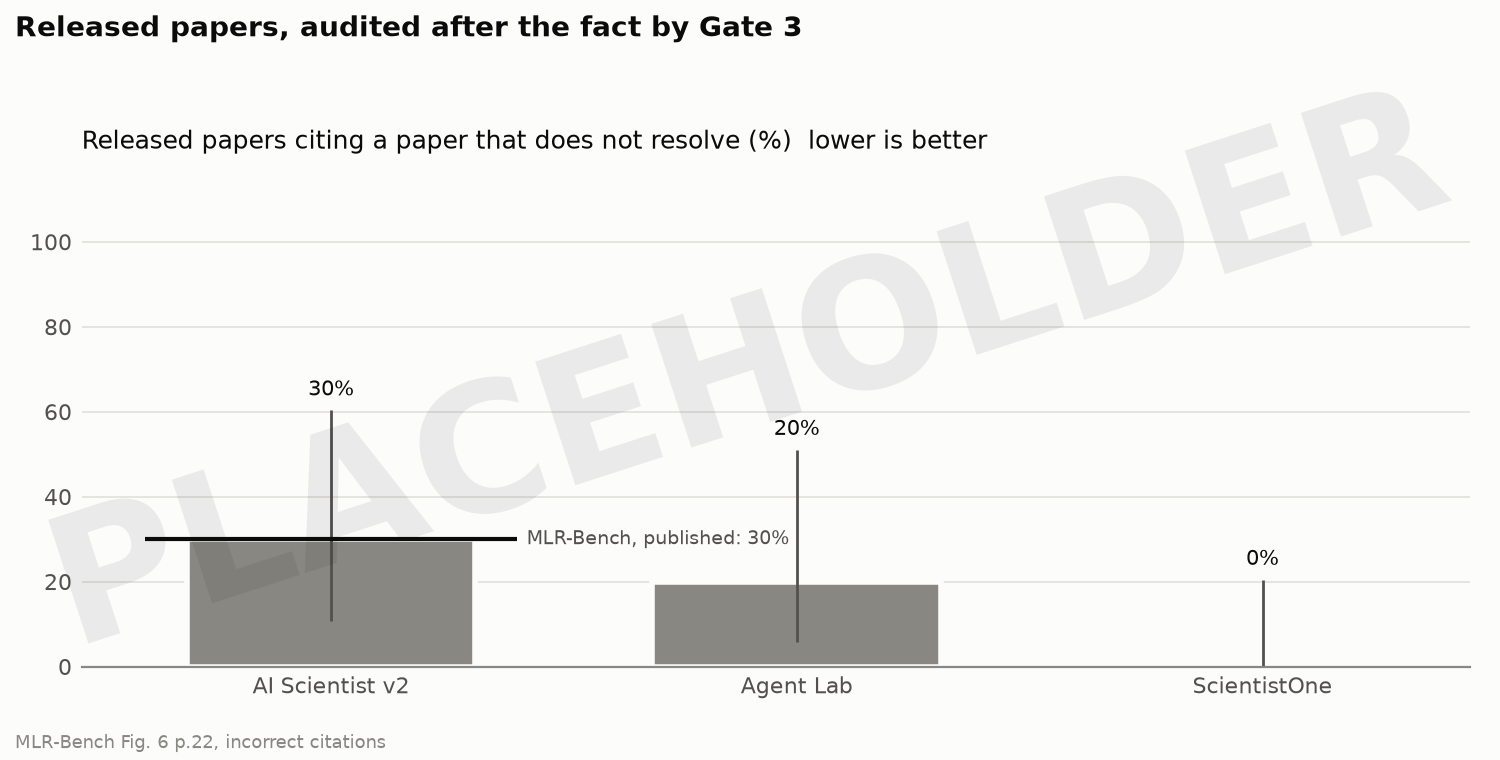
\includegraphics[width=0.6\textwidth]{../figures/fig7_audit.png}
\caption{Released papers, audited after the fact with Gate 3's citation check.}
\label{fig:audit}
\end{figure*}

\paragraph{Released papers.}
\todo{Figure~\ref{fig:audit}. The two published figures for AI Scientist-v2 disagree: MLR-Bench reports incorrect citations in 30\% of its papers, ScientistOne 0 of 159 hallucinated references on different tasks.}

\section{Limitations}

The gates deliver the evidence; they do not make the science good.
In the Gate 1 campaign, reviewer scores were 3.735 gated and 3.765 ungated, and both papers were recommended for rejection.
Gate 2's methodology checks read plan fields a model extracts from free-text plans, so a divergence on one is capped at a warning.
\todo{Whatever the runs show.}

\section{Conclusion}

\todo{After results.}

\bibliographystyle{ACM-Reference-Format}
\bibliography{refs}

\appendix

\section{Mechanism Evidence}

These results measure how the gates behave, and are already in the repository.

\begin{table}[h]
\caption{Measured mechanism results.}
\begin{tabular}{p{0.16\columnwidth}p{0.74\columnwidth}}
\toprule
Gate & Result \\
\midrule
1 & 40/40 required values reached the writer, against 0/40 through a 1,000-character channel \\
1 & 28/29 manuscript claims traceable, against 0/11 ungated \\
2, tier A & 27/27 defects caught, 0/18 clean registries flagged \\
2, tier B & 12/12 and 6/6 caught, 0/17 and 0/23 false alarms \\
3 & 34 of 49 result literals detected in two archived manuscripts \\
\bottomrule
\end{tabular}
\end{table}

\begin{figure*}[t]
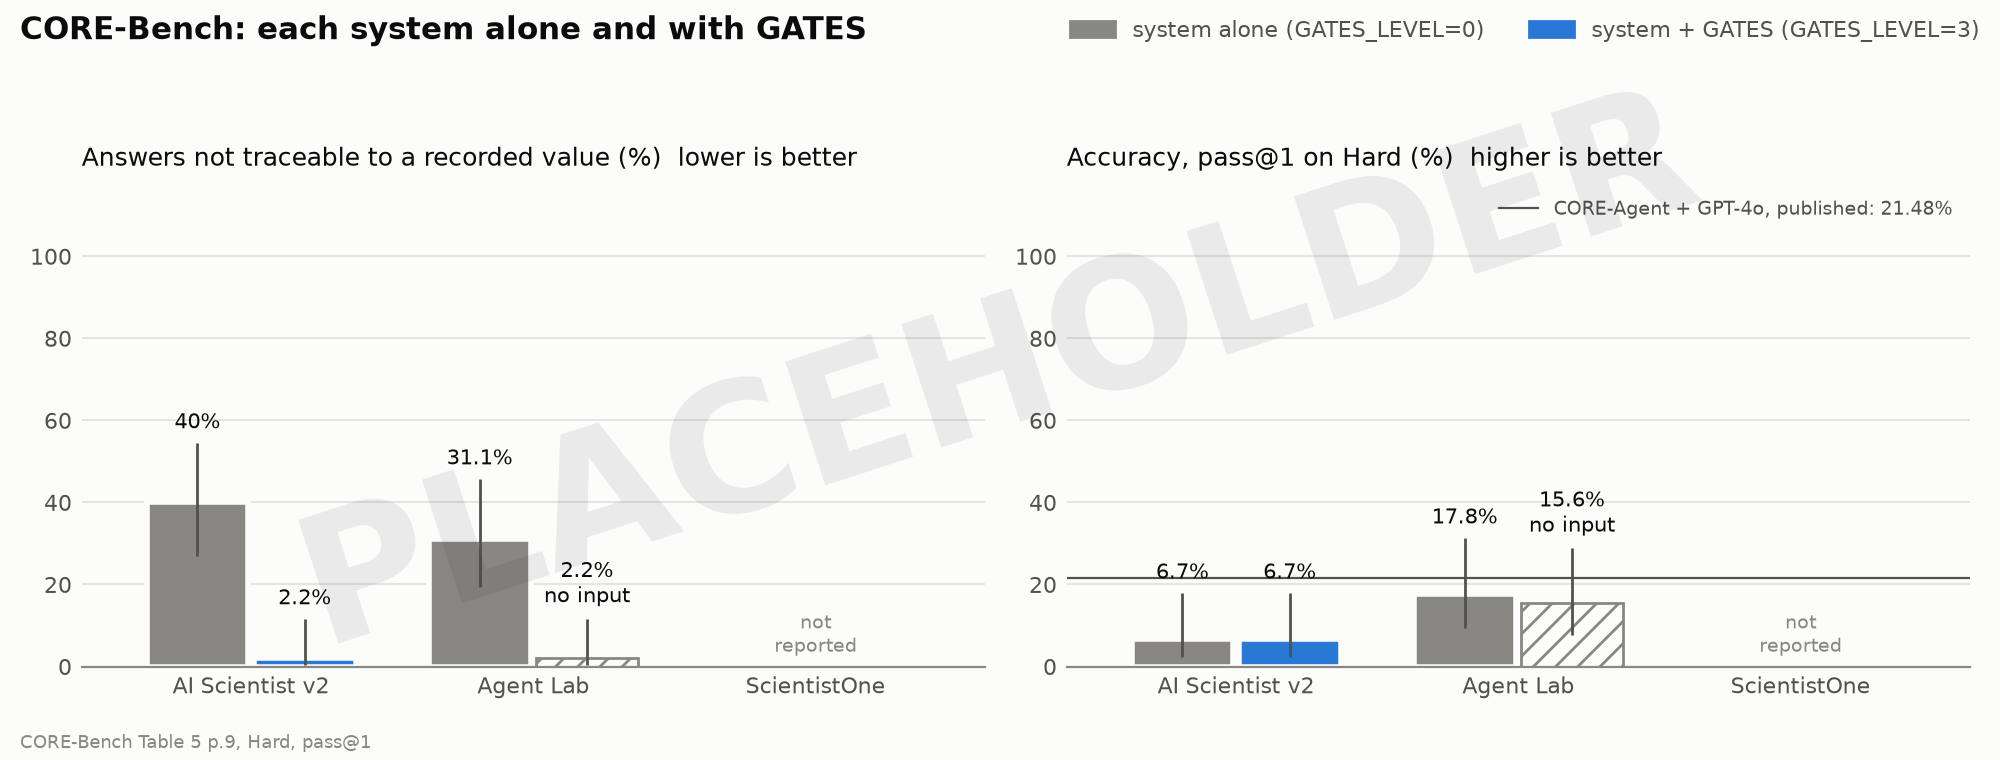
\includegraphics[width=\textwidth]{../figures/fig4_corebench_compare.png}
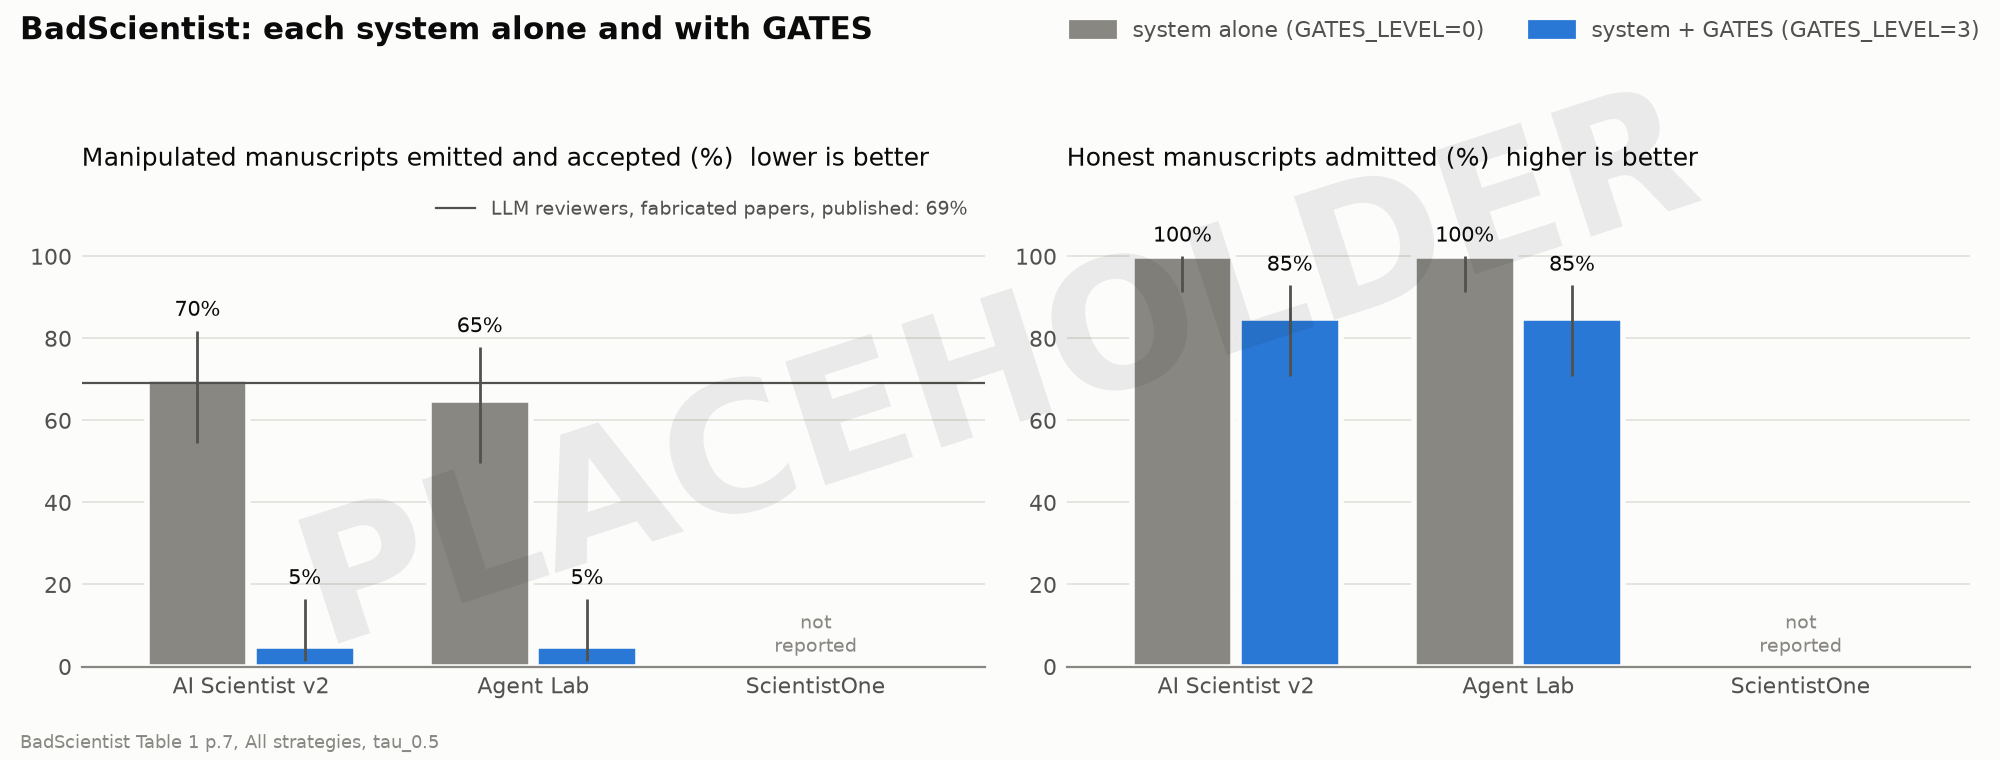
\includegraphics[width=\textwidth]{../figures/fig6_badscientist_compare.png}
\caption{Each system alone and with \gates{}, on CORE-Bench and BadScientist.}
\end{figure*}

\end{document}
